\documentclass[11pt, oneside]{article}  
\usepackage[margin=1in]{geometry}     
\geometry{letterpaper}                   	
\usepackage{graphicx}			
\usepackage{amssymb}
\usepackage{amsmath}
\usepackage[usenames,dvipsnames,svgnames,table]{xcolor}
\usepackage{multicol}

\title{Stat, fast}
\author{(I already said that)} %Schwartz
\setcounter{section}{-1}

\begin{document}
\maketitle

\section{Synopsis}
Come ready to be put on the spot. You'll be less put on the spot if you know the following.

\section{Probs}

\begin{minipage}{0.4\linewidth} 
\begin{itemize}
\item {[}Permut/Combin{]}ation
% P: n!/(n-k)! -- all possible orderings
% C: n!/((n-k)!k!) -- all possible groupings
\item Choose
% what is it and which of the above is it?
\item[] ${}$
\item Random Variables
% Sample space, outcomes, events
\item Discrete Distributions
% Look them up: Bernoulli, Binomial (multinomial), Geometric, Poisson (binomial approximation; X+Y)
\item Continuous Distributions
% Look them up: Uniform, Normal (X+Y), Gamma (exponential (aging property), chi-squared), beta
\end{itemize}
\end{minipage}
\begin{minipage}{.65\linewidth} 
\begin{itemize}
\item Joint Distributions
% vectors as opposed to scalars, chain rule, distribution
\item $\textrm{E}[aX], \textrm{Var}[X], \textrm{E}[XY+Z]$ and $\textrm{Var}[aX+bY]$
% define these and formulas
\item Covariance Vs Correlation Vs Causation
% define, association !=0 causal -- this is *linear association* (figure of this last fact)
\item[] Vs Independent Vs Mutually Exclusive
% Contrast
\item Bayes' Theorem
% Likelihood, Prior, marginal likelihood
% LotP=marginalization: marginal likelihood, normalizing constant
\item \textcolor{gray}{Standard Error $\downarrow$} 
% Define se, CLT, Bias vs Variance
\end{itemize}
\end{minipage}

\section{Inf(erence)}

\begin{minipage}{.15\linewidth}
\begin{itemize}
\item MLE
% likelihood a function of the parameter given the data -- do a coin flipping example
% compare to MoM
\item CLT
% what it is yo -- ASSUMPTIONS? iid, "large enough'' sample size
\end{itemize}
\end{minipage}
\begin{minipage}{.85\linewidth}
\begin{itemize}
\item Bootstrapping Vs Bayes 
% what it is yo -- distribution approximation
% compare it to Bayes
% when to use?
\item[] Vs Confidence Intervals Vs Nonparametric (NP) estimation \textcolor{gray}{Vs NP tests  $\downarrow$}
% repeated throwing of confidence intervals
% compare Bayesian confidence intervals to Bootstrapped intervals
% NP: less assumptions that can be errors... less power gained from assumptions... 
% allows for unique distributions not well modeled by parametric forms... 
% kernel density estimation versus parametric distribution estimation
% testing is different e.g., mann whitney test
\end{itemize}
\end{minipage}

\section{Testing}

\begin{minipage}{.5\linewidth}
\begin{itemize}
\item $\emptyset$ Vs $H_a$
% what are they?
\item $p$ Vs $\alpha$ Vs Type II 
% define, -value vs significance level versus 1-Power
% one-sided vs two-sided
% measure of evidence -- only good for alpha
% Not at all probability of null being true (cuz it is/isn't and the frequentist world doesn't estimate that -- bayes does)
% [there's not a random even with probability sometimes H_0 true, etc. ]
% Not at all probability of making an error (that's alpha)
% POWER ANALYSIS -- say in a normal case
\item Multiple testing correction via Bonferroni 
\item[] {[}Vs False Discovery Rate (FDR){]}
% what is the issue with multiple testing?
\end{itemize}
\end{minipage}
\begin{minipage}{.25\linewidth}
\begin{itemize}
\item (A/B) $t$-test
% independent, (un)equal variance, paired
% npq -- why? 
% degrees of freedom and z-tests and assumptions
% one versus two sided
\item $\chi^2$-test
% df = (r-1)*(c-1)
% E_r,c = (n_r)*(n_c)/n
% X2 = sum (O_r,c - E_r,c)^2/E_r,c
\item $X+Y \sim$ ?
% *NOT* a mixture-model
% functionals 
\item \textcolor{gray}{Bayes $\downarrow$}
% contrast with how would bayes do this? They would say Pr(something)
\end{itemize}
\end{minipage}


\section{Multi-armed Bandit}
% difference to Bayes discussed above
% posteriors/((non-)conjugate,(im)proper,flat,uniform,jeffrey's,(non-)informative)priors/likelihood discussed below
\begin{itemize}
\item Ready, go
% and tell me about it: softmax, ucb1, epsilon-greedy, bayesian (max, random)
% regret
\end{itemize}


\section{Bayes}
% automatic multiple testing adjustment via Bayesian hierarchical model 
% multiple testing problem 
% false discovery rate model

% say something about conjugate forms here
% say something about one sided tests here

We are monitoring credit card (cc) purchases for fraud by testing a measure of ``unusual purchases''.\\

Let $\pi$ denote the overall fraud rate (for which we may have some prior belief), 

$$ \left\{  \begin{array}{ll} 
    f_i=1: & \textrm{if there is in fact fraud for cc $i$, and} \\
    f_i=0: & \textrm{if not,} 
   \end{array} \right.$$

\noindent and $t_i$ be our ``unusual purchases'' measure which will depend on $f_i$.  That is, 

\begin{align*}
d(\pi) \propto{}& \pi^{\alpha-1}(1-\pi)^{\beta-1} \\
p(f_i|\pi) ={}& \pi^{f_i}(1-\pi)^{(1-f_i)}  \\
t_i|f_i \sim{}& d_{f_i}(t_i) 
\end{align*}


\noindent so that (upon marginalizing out the latent fraud indicator $f_i$) the measures $t_i$ are generated from a mixture distribution of fraudulent $d_{1}$ and genuine $d_{0}$ cc purchases, i.e., 

\begin{align*}
d(t_i|\pi) ={}& (1-\pi)d_{0}(t_i) + \pi d_{1}(t_i)  
\end{align*}

\vspace{-1.5em}
\begin{figure}[h!]
   \centering
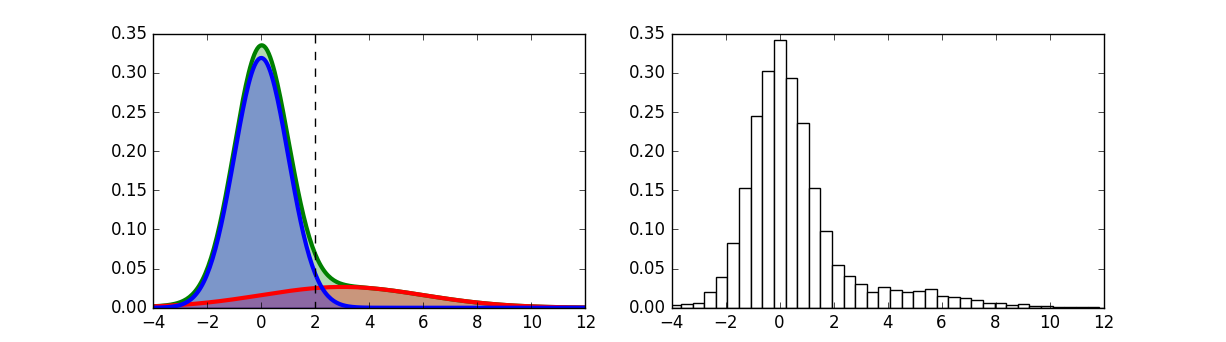
\includegraphics[width=7in]{fraud.png}  
\end{figure}  

\noindent and we are interested in 

\begin{minipage}{.49\linewidth}
\begin{align*} 
     {}& p(f_i=1|t_1,\cdots t_n,f_1,\cdots f_{i-1},f_{i+1},\cdots f_{n}) \\
     \propto{}& \prod d_{f_i}(t_i)p(f_i|\pi) \cdot d(\pi) \\
    \propto{}& d_{1}(t_i) \int \pi^{1+\underset{j \not = i}{\sum}f_j + \alpha-1}(1-\pi)^{
    \underset{j \not = i}{\sum} (1-f_j) +  \beta-1} d\pi \\
    \approx{}& d_{1}(t_i)  \hat \pi \\
    {}\\
{}& p(f_i=0|t_1,\cdots t_n,f_1,\cdots f_{i-1},f_{i+1},\cdots f_{n})  \\
\propto{}& \prod d_{f_i}(t_i)p(f_i|\pi)  \cdot  d(\pi) \\
   \propto{}& d_{0}(t_i) \int \pi^{\underset{j \not = i}{\sum}f_j + \alpha-1}(1-\pi)^{
    1+\underset{j \not = i}{\sum} (1-f_j) +  \beta-1} d\pi   \\
      \approx{}& d_{0}(t_i)  (1-\hat \pi) \\
   \end{align*}
\end{minipage}
\begin{minipage}{.35\linewidth}
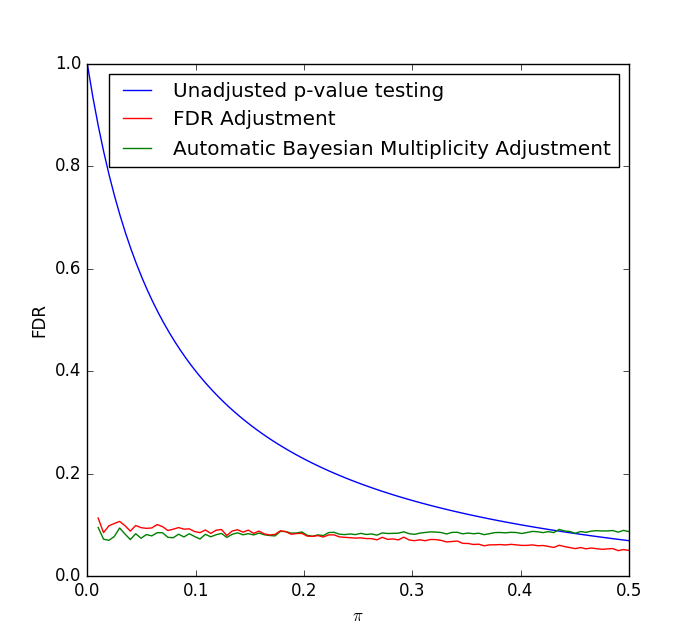
\includegraphics[width=3.15in]{bayesAutoMultAdj.png}
\end{minipage}

\begin{verbatim}
False Discovery Rate (FDR), see: statsmodels.sandbox.stats.multicomp.fdrcorrection0
\end{verbatim}

\section*{Appendix: n-1?}

\begin{minipage}{.375\linewidth} 

   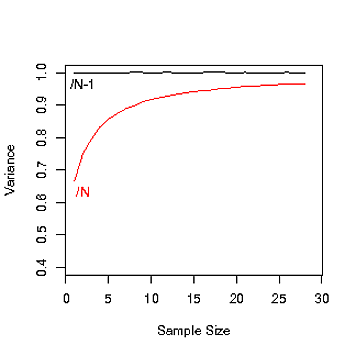
\includegraphics[width=2.5in]{fZcgG.png}  
   
   Dividing by $(n-1)$ rather than $n$ results in an unbiased estimator of $\sigma^2$\\

\end{minipage}
\begin{minipage}{.05\linewidth}
${}$
\end{minipage}
\begin{minipage}{.625\linewidth} 
\begin{align*} 
\textcolor{white}{=} {}& E\left[\sum_{i=1}^n\left(x_i^2-\frac{1}{n}\sum_{j=1}^nx_j\right)^2\right] \\
= {}& E\left[\sum_{i=1}^n\left(x_i^2-\frac{2x_i}{n}\sum_{j=1}^nx_j + 
\left(\frac{1}{n}\sum_{j=1}^nx_j\right)^2\right)\right] \\ 
= {}& E\left[\sum_{i=1}^nx_i^2-\textcolor{blue}{\frac{2}{n} \sum_{i=1}^n \sum_{j=1}^nx_ix_j} + 
\textcolor{red}{\frac{1}{n} \sum_{i=1}^n\sum_{j=1}^nx_ix_j}\right] \\ 
= {}& E\left[\sum_{i=1}^nx_i^2 - \textcolor{blue}{\frac{2}{n}\sum_{i=1}^nx_i^2 -\frac{2}{n}\sum_{j\not=i}x_ix_j} + 
\textcolor{red}{\frac{1}{n}\sum_{i=1}^nx_i^2 + \frac{1}{n}\sum_{j\not=i}x_ix_j} \right] 
\end{align*}
\end{minipage}

\begin{align*}
= E\left[\sum_{i=1}^nx_i^2 - \textcolor{blue}{\frac{2}{n}\sum_{i=1}^nx_i^2} + \textcolor{red}{\frac{1}{n}\sum_{i=1}^nx_i^2} 
 -\textcolor{blue}{\frac{2}{n}\sum_{j\not=i}x_ix_j}  
 + \textcolor{red}{\frac{1}{n}\sum_{j\not=i}x_ix_j} \right] 
 = {}& E\left[\textcolor{black}{\frac{n-1}{n}\sum_{i=1}^nx_i^2} 
 -\textcolor{black}{\frac{1}{n}\sum_{j\not=i}x_ix_j}  \right] \\  
 = {}& \textcolor{black}{\frac{n-1}{n}\sum_{i=1}^n E\left[x_i^2\right] } 
 -\textcolor{black}{\frac{1}{n} \sum_{j\not=i} E\left[x_ix_j\right] }   \\ 
 = {}& \textcolor{black}{\frac{n-1}{n}\sum_{i=1}^n (\sigma^2 + \mu^2) } 
 -\textcolor{black}{\frac{1}{n} \sum_{j\not=i} \mu^2 } \quad (\emph{\textrm{why?}})  \\ 
 = {}& \textcolor{black}{(n-1) (\sigma^2 + \mu^2) } 
 -\textcolor{black}{\frac{n^2-n}{n} \mu^2 }   =  \textcolor{violet}{(n-1)\sigma^2}
\end{align*}


\section*{Appendix: uncorrelated $\overset{\Longrightarrow}{\underset{\Longleftarrow}{?}}$ independent \emph{hint}}

\begin{figure}[h] 
   \centering
   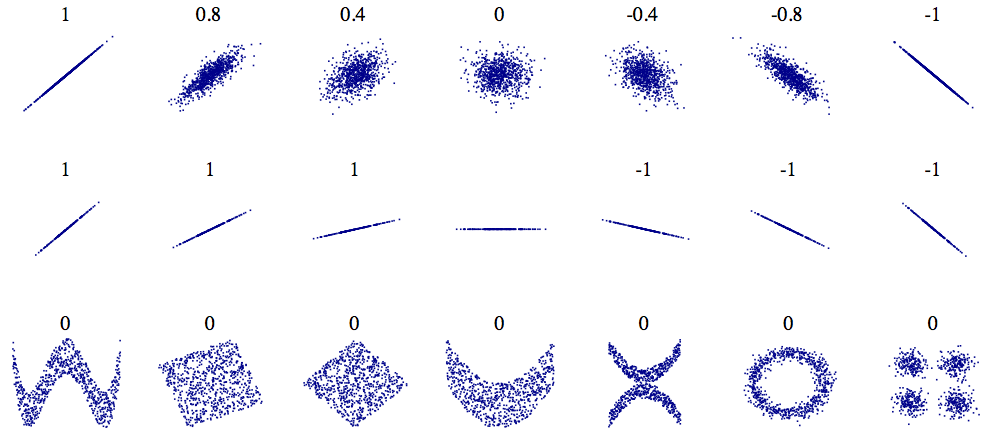
\includegraphics[width=5.5in]{cors.png}  
\end{figure}  

\end{document}  
